\section{Zielsetzung}
Durch Messung der Transmission von Licht durch Rubidiumgas bei Anlegen eines externen Magnetfeldes werden die
Stärke des Erdmagnetfeldes, die Lande-Faktoren und die Spins der Elektronenhülle und des Kerns der Rubidiumisotope
Rb-85 und Rb-87 berechnet.
Für die beiden verwendeten Rubidiumisotope sind Hyperfeinstruktur- und Zeeman-Aufspaltung unterschiedlich. Die damit
verbundenen Kenngrößen - der Landefaktor, das gyromagnetische Verhältnis und der Spin - können mit Hilfe optischen
Pumpens aufgrund der unterschiedlichen Enerdifferenzen sehr präzise gemessen werden.

\section{Theorie}

\subsection{Aufspaltung von Energieniveaus}

Quantenzahlen beschreiben Zustand eines atomareb Systems.
Das magnetische Moment der gesamten Elektronenhülle $\vec{J}$ setzt sich aus den magnetischen Momenten von
Bahndrehimpuls $\vec{L}$ und Spin $\vec{S}$ zusammen:
\begin{equation}
  \vec{\mu}_\text{J} = \vec{\mu}_\text{L} + \vec{\mu}_\text{S} \quad \text{mit} \quad |\vec{\mu}_\text{J}| = \mu_\text{B}\sqrt{L (L + 1)} \quad \text{und}
  \quad |\vec{\mu}_\text{S}| = g_\text{S}\mu_\text{B}\sqrt{S (S + 1)}.
\end{equation}
Der Gesamtdrehimpuls der Elektronenhülle $\vec{J}$ ist über
\begin{equation}
  \vec{\mu}_\text{J} = -g_\text{J}\mu_\text{B}\vec{J} \quad \text{bzw.} \quad |\vec{\mu}_\text{J}| = -g_\text{J}\mu_\text{B}\sqrt{J (J + 1)}
  \label{magnMom}
\end{equation}
mit einem magnetischen Moment verknüpft, dabei ist $\mu_\text{B}$ das Bohrsche Magneton.
$g_\text{S}$ ist der Lande-Faktor des freien Elektrons, der Zusammenhang der magnetischen Momente wird durch den
Lande-Faktor $g_\text{J}$ ausgedrückt.
%$\vec{\mu}_J$ präzediert um $\vec{J}$, sodass für den Betrag gilt:
%\begin{align}
%  \begin{split}
%    |\vec{\mu}_J| &= |\vec{\mu}_L|\cos\beta + |\vec{\mu}_S|\cos\alpha\\
%    \equiv g_J\mu_B\sqrt{J (J + 1)} = & \mu_B\sqrt{L (L + 1)}\cos\beta + g_S\mu_B\sqrt{S (S + 1)}\cos\alpha
%  \end{split}
%\end{align}
Dieser kann aus den Quantenzahlen über
\begin{equation}
  g_\text{J} = \frac{3.0023J(J+1) + 1.0023[S(S+1) - L(L+1)]}{2J(J+1)}
\end{equation}
berechnet werden.

Der sogenannte Zeeman-Effekt beschreibt die Aufspaltung in $2J+1$ Energieniveaus bei Anlegen eines äußeren
Magnetfeldes. Liegt ein äußeres Magnetfeld $\vec{B}$ an, kommt es zu einer Aufspaltung der durch $L$, $S$ und
$J$ definierten Feinstruktur-Energieniveaus, da das magnetische Moment $\vec{\mu}$ mit dem Feld wechselwirkt; die
Wechselwirkungsenergie ist
\begin{equation}
  U_\text{magn} = -\vec{\mu}_\text{J}\cdot\vec{B}.
\end{equation}
Da nur die zu $\vec{B}$ parallele Komponente des magnetischen Moments zu diesem Effekt beiträgt, kommt es zu einer Aufspaltung
der Energieniveaus gemäß
\begin{equation}
  U_\text{magn} = M_\text{J}g_\text{J}\mu_\text{B}B,
\end{equation}
wobei $M_\text{J}$ ganzzahlig ist und aus $-J, -J+1, ..., J-1, J$ stammt.

Bei einem nicht-verschwindenden Kernspin $\vec{I}$ kommt es zudem zu einer Aufspaltung in Hyperfeinstrukturniveaus.
Der Gesamtdrehimpuls der Elektronenhülle $\vec{J}$ koppelt an den Drehimpuls des Kerns $\vec{I}$ zum Gesamtdrehimpuls des Atoms
\begin{equation}
  \vec{F} = \vec{J} + \vec{I}.
\end{equation}
Die Energiedifferenz benachbarter Zeeman-Niveaus ist dann
\begin{equation}
  U_\text{UF} = g_\text{F}\mu_\text{B}B.
\end{equation}
Der Lande-Faktor ist in diesem Fall
\begin{equation}
  g_\text{F} \approx g_\text{J}\frac{F(F+1)+J(J+1)-I(I+1)}{2F(F+1)}.
\end{equation}
$F$ läuft von $I+J$ bis $|I-J|$, jedes Hyperfeinniveau spaltet in einem äußeren Magnetfeld in weiter $2F+1$ Zeeman-Niveaus
auf. Für ein Alkali-Atom mit $I=\frac{3}{2}$ ist dies in \autoref{aufspaltung} beispielhaft gezeigt.
\begin{figure}
  \centering
  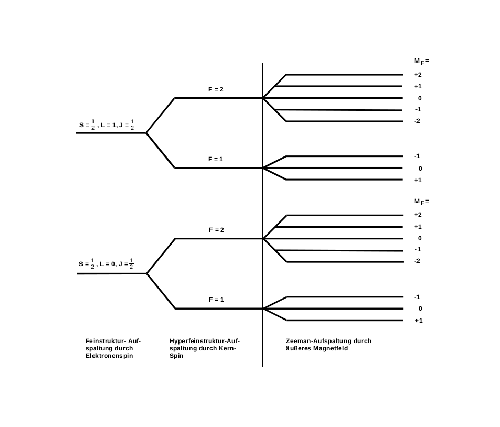
\includegraphics[width=\textwidth]{img/aufspaltung.pdf}
  \caption{Feinstruktur-, Hyperfeinstruktur- und Zeeman-Aufspaltung, beispielhaft für ein Alkali-Atom mit
  $I=\frac{3}{2}$.}
  \label{aufspaltung}
\end{figure}

\subsection{Optisches Pumpen}

Die Energieniveaus der inneren Schalen der Elektronenhülle sind vollstandig besetzt, die Besetzung der äußeren Schalen ist
temperaturabhängig. Im thermischen Gleichgewicht wird sie für zwei Niveaus mit den Energien $W_1$ und $W_2$ durch die
Boltzmannsche Gleichung
\begin{align}
  \frac{N_2}{N_1} = \frac{g_2}{g_1}\frac{\exp(-W_2/kT)}{\exp(-W_1/kT)}
  \label{boltz}
\end{align}
beschrieben. $N_i$ sind die Besetzungszahlen der jeweiligen Zustände und die statistischen Gewichte $g_i$ sind ein Maß
dafür, wie viele Zustände es pro Energie $W_i$ gibt.

Der Begriff Optisches Pumpen bezeichnet eine Methode, mit der eine Abweichung von der in \autoref{boltz} gegebenen
Verteilung erzielt werden kann - zum Beispiel in Form einer Inversion, bei der $N_2 > N_1$ gilt.
Dafür wird Licht eingestrahlt, das gerade die nötige Energie besitzt, um ein Hüllenelektron vom Grundzustand in einen
angeregten Zustand zu versetzen. Für ein Alkali-Atom mit $J=\frac{1}{2}$ beispielsweise kann $M_\text{J}$ also nur
$\pm \frac{1}{2}$ werden.
Da bei der Absorption und Emission eines Photons Drehimpulserhaltung gelten muss, sind nur bestimmte Übergänge
zwischen unterschiedlichen Energieniveaus möglich; Ddiese Übergänge sind über Auswahlregeln definiert.
Aufgrund dieser Auswahlregeln sind nur Übergänge mit $\Delta M = 0,\pm 1$ möglich.
Bei $\pi$-Übergangen mit $\Delta M = 0$ wird linear polarisiertes Licht emitiert und absorbiert, für $\sigma^\pm$-Übergänge
mit $\Delta M = \pm 1$ ist es rechtszirkular- bzw. linkszirkular-polarisiertes Licht.
Wird rechtszirkular-polarisiertes Licht in eine Zelle mit verdampftem Rubidium eingestrahlt, können aufgrund der
Beschränkung $\Delta M_\text{J} = 1$ nur Elektronen aus dem energetisch niedrigeren Grundzustand angeregt werden.
Durch spontane Emission aus dem angeregten Zustand, werden aber beide Grundzustände bevölkert. Das energieärmere
Niveau wird fortlaufend durch Einstrahlung von Licht geleert, das energetisch höhere, aus dem keine Elektronen
angeregt werden können, wird gesättigt. Als Resultat steigt die Transmission mit der Zeit asymptotisch gegen den
Wert 1, da keine Elektronen mehr verfügbar sind, die angeregt werden können.

\subsection{Messung der Zeeman-Aufspaltung}

Ein Elektron im angeregten Zustand kann durch spontane oder durch angeregte Emission in seinen Grundzustand zurückkehren.
Dabei ist letzteres bei Energien, die für Zeeman-Aufspaltung relevant sind, um 25 Größenordnungen wahrscheinlicher, da die
Übergangswahrscheinlichkeit für spontane Emission $\propto \nu^3$ ist.
Die Zeeman-Aufspaltung tritt nur bei angelgtem Magnetfeld auf, sodass auch nur bei externem Magnetfeld das optische Pumpen
durch Einstrahlen einer geeigneten Lichtquelle in stattfinden kann. Wird ein Magnetfeld angelegt, dass das Erdmagnetfeld gerade ausgleicht, findet keine Aufspaltung statt,
es tritt keine Inversion auf und der Transmissionskoeffizient sinkt.
Ein solcher Einbruch in der Intensität des Lichts tritt auch auf, wenn ein frequenzvariables Hochfrequenzfeld an die
Dampfzelle angelegt wird. Das Magnetfeld wird variiert und sobald es den Wert
\begin{equation}
  B_\text{m} = \frac{4\pi m_0}{\text{e}_0g_\text{J}}\nu
\end{equation}
erreicht, setzt induzierte Emission ein. Die Inversion wird aufgehoben, das eingestrahlte Licht kann wieder absorbiert werden
und der Transmissionskoeffizient fällt ab. Die geschieht jeweils für die beiden Rubidiumisotope bei unterschiedlichem
Magnetfeld.

\subsection{Quadratischer Zeeman-Effekt}

Wird die magnetische Flussdichte vergrößert, müssen bei der Berechnung der Übergangsenergie Terme höherer Ordnung von $B$
berücksichtigt werden, da nun die Spin-Bahn-Wechselwirkung relevant wird. Die Zeeman-Übergänge haben eine unterschiedliche
Energie und sind abhängig von $M_\text{F}$. Der Übergang von einem Zustand $M_\text{F}$ zu $M_\text{F}-1$ mit einer
Hyperfeinstrukturaufspaltung $\Delta E_\text{Hy}$ wird durch die Breit-Rabi-Formel beschrieben:
\begin{equation}
  U_\text{HF} = g_\text{F}\mu_\text{B}B + {g_\text{F}}^2{\mu_\text{B}}^2B^2\frac{1-2M_\text{F}}{\Delta E_\text{Hy}}
\end{equation}

\subsection{Transiente Effekte}

Wird das Hochfrequenzfeld schnell ein- und ausgeschaltet, präzediert der Kernspin um das effektive Magnetfeld. Die
Lamor-Frequenz $\\nu = \gamma B_\text{RF}$ mit dem gyromagnetischen Verhältnis $\gamma = g_\text{f}\frac{\mu_ß}{\text{h}}$
ist vom Lande-Faktor abhängig und somit für die beiden Rubidiumisotope verschieden. Das Verhältnis der Relaxationsperioden
$T = 1/\gamma B_\text{RF}$ ist dann
\begin{equation}
  \frac{T_{87}}{T_{85}} = \frac{\gamma_{85}}{\gamma_{87}}.
\end{equation}
